
\documentclass{beamer}

\mode<presentation>
\usetheme{bbk2}
\usefonttheme{structurebold}
\usepackage{graphicx,epstopdf}
\usepackage{tikz}
\usepackage{multirow}
\usepackage[skins,theorems]{tcolorbox}
\usepackage[dvipsnames]{xcolor}


\usetikzlibrary{graphs}
\usetikzlibrary{graphs.standard}

\begin{document}
\title[Galois Groups of Chromatic Polynomials of Some Generalised Theta Graphs]{Galois Groups of Chromatic Polynomials of Some Generalised Theta Graphs}
\author[xud]{xud}

\institute[Матклуб]{Матклуб}
\date{}
\begin{frame}
\titlepage
\end{frame}


\begin{frame}
\frametitle{What is a Chromatic Polynomial?}
\begin{definition}[Graph]
A graph G(V,E) is a finite nonempty set V and a set E of
subsets of V of size two. The elements of V are called \textbf{vertices} and the elements of E are called \textbf{edges}
\end{definition}
\begin{center}
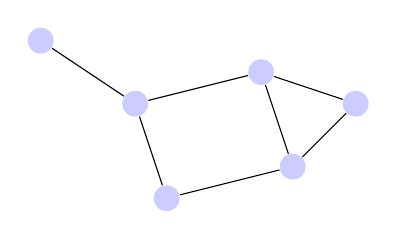
\begin{tikzpicture}
  [scale=.4,auto=left,every node/.style={circle,fill=blue!20}]
  \node (n6) at (1,10) {};
  \node (n4) at (4,8)  {};
  \node (n5) at (8,9)  {};
  \node (n1) at (11,8) {};
  \node (n2) at (9,6)  {};
  \node (n3) at (5,5)  {};

  \foreach \from/\to in {n6/n4,n4/n5,n5/n1,n1/n2,n2/n5,n2/n3,n3/n4}
    \draw (\from) -- (\to);
\end{tikzpicture}

\end{center}

\textbf{Chromatic polynomials} are an object of study of \textbf{Algebraic Graph Theory}, which is the study of graphs using algebraic methods.
\end{frame}


\begin{frame}
\frametitle{What is a Chromatic Polynomial?}
\alert{Approach:} Define an (algebraic) invariant of a graph and study it using algebraic (and/or analytic) methods

\begin{definition}[Proper colouring of a graph]
A proper colouring of a graph is painting all the vertices of a graph with colours such that no two adjacent vertices have the same colour
\end{definition}

%\begin{center}



\begin{columns}
\begin{column}{5cm}
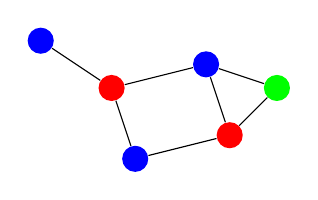
\begin{tikzpicture}
  [scale=.3,auto=left,every node/.style={circle,fill=blue!20}]
  \node (n6) at (1,10) [fill=blue] {};
  \node (n4) at (4,8)  [fill=red] {};
  \node (n5) at (8,9)  [fill=blue] {};
  \node (n1) at (11,8) [fill=green] {};
  \node (n2) at (9,6)  [fill=red] {};
  \node (n3) at (5,5)  [fill=blue] {};

  \foreach \from/\to in {n6/n4,n4/n5,n5/n1,n1/n2,n2/n5,n2/n3,n3/n4}
    \draw (\from) -- (\to);
\end{tikzpicture}
\end{column}
\begin{column}{5cm}
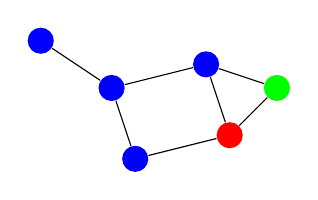
\begin{tikzpicture}
  [scale=.3,auto=left,every node/.style={circle,fill=blue!20}]
  \node (n6) at (1,10) [fill=blue] {};
  \node (n4) at (4,8)  [fill=blue] {};
  \node (n5) at (8,9)  [fill=blue] {};
  \node (n1) at (11,8) [fill=green] {};
  \node (n2) at (9,6)  [fill=red] {};
  \node (n3) at (5,5)  [fill=blue] {};

  \foreach \from/\to in {n6/n4,n4/n5,n5/n1,n1/n2,n2/n5,n2/n3,n3/n4}
    \draw (\from) -- (\to);
\end{tikzpicture}
\end{column}
\end{columns}

%\end{center}

\begin{definition}[Preliminary: P(G,k)]
For a graph G, let P(G,k) define the \textbf{function}, giving the number of proper colourings of the graph G with k colours
\end{definition}
\end{frame}


\begin{frame}
\frametitle{What is a Chromatic Polynomial?}
\alert{Simple example:} 
\begin{columns}
\begin{column}{4cm}
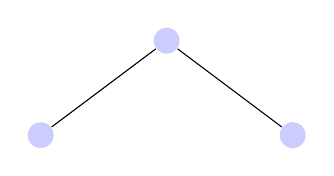
\begin{tikzpicture}
  [scale=.4,auto=left,every node/.style={circle,fill=blue!20}]
  \node (n1) at (1,5) {};
  \node (n2) at (5,8)  {};
  \node (n3) at (9,5)  {};
%  \node (n1) at (11,8) {};
%  \node (n2) at (9,6)  {};
%  \node (n3) at (5,5)  {};

  \foreach \from/\to in {n1/n2,n2/n3}
    \draw (\from) -- (\to);
\end{tikzpicture}
\end{column}
\begin{column}{2cm}
\begin{align*}
   k &=& 1 \\
   k &=& 2 \\
   k &=& 3 \\
         &\vdots& \\
   k &=& N
\end{align*}
\end{column}

\begin{column}{2cm}
\begin{align*}
   P(G,1) &=& 0 \\
   P(G,2) &=& 2 \\
   P(G,3) &=& 12 \\
         &\vdots& \\
   P(G,N) &=& N(N-1)^2
\end{align*}
\end{column}
\end{columns}

\begin{theorem}
P(G,k) is a polynomial.
\end{theorem}

\begin{definition}[Chromatic Polynomial P(G,k)]
For a graph G, let P(G,k) define the \textbf{polynomial}, giving the number of proper colourings of the graph G with k colours
\end{definition}
\end{frame}



\begin{frame}
\frametitle{A more intriguing example: Petersen Graph}
\begin{center}

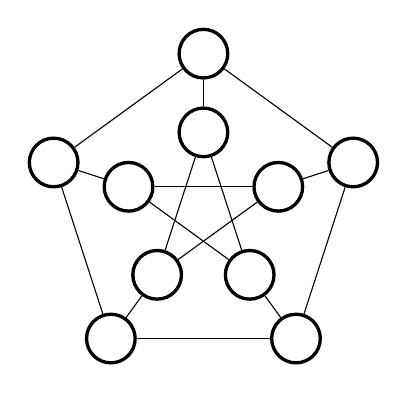
\begin{tikzpicture}[every node/.style={draw,circle,very thick, text=white}]
  \graph[clockwise, radius=2cm] {subgraph C_n [n=5,name=A]};
  \graph[clockwise, radius=1cm] {subgraph I_n [n=5,name=B]};

  \foreach \i in {1,2,3,4,5}{\draw (A \i) -- (B \i);}
  \newcounter{j}
  \foreach \i in {1,2,3,4,5}{%
  \pgfmathsetcounter{j}{ifthenelse(mod(\i+2,5),mod(\i+2,5),5)}
  \draw (B \i) -- (B \thej);
  }
\end{tikzpicture}

\(P(G,k) = k(k-1)(k-2)(k^7-12k^6+67k^5-230k^4+529k^3-814k^2+775k-352)\)

\begin{theorem}
For a Graph G on n vertices, P(G,k) is a \textbf{monic} polynomial of degree exactly n with \textbf{integer coefficients}.
\end{theorem}

\end{center}
\end{frame}


\begin{frame}
\frametitle{Recap of main terms}
\begin{definition}[Proper colouring of a graph]
A proper colouring of a graph is painting all the vertices of a graph with colours such that no two adjacent vertices have the same colour
\end{definition}
\begin{definition}[P(G,k)]
For a graph G, let P(G,k) define the \textbf{function}, giving the number of proper colourings of the graph G with k colours
\end{definition}
\begin{theorem}
For a Graph G on n vertices, P(G,k) is a \textbf{monic} polynomial of degree exactly n with \textbf{integer coefficients}. Hence we will refer to P(G,k) as the \textbf{chromatic polynomial of graph G}.
\end{theorem}

\end{frame}

\begin{frame}
\frametitle{Key concepts from Galois theory [1]}
Given a polynomial $p(x) = a_0+a_1x+a_2x^2+...+a_nx^n$ what can we say about the set of its roots? Also: what can we say about how it factors?
\\
That depends on over which field this is being considered. We know that over $\mathbb{C}$ it will factor into n linear factors (or - equivalently - will have n complex roots), but over $\mathbb{Q}$ that may not be the case.
\begin{definition}[Splitting field of a polynomial]
Let $F$ be a field and let $p$ be a polynomial in $F[x]$ of degree $\ge 1$. By a splitting field $K$ of p we shall mean an extension K of F such that p splits into linear factors in K, i.e. $p(x) = c(x-\alpha_1)...(x-\alpha_n)$, where $\alpha_i \in 
 K, i=1,...,n$, and such that $K=F(\alpha_1,...,\alpha_n)$ is generated by all the roots of p. 
\end{definition}

\end{frame}

\begin{frame}
\frametitle{Key concepts from Galois theory [2]}
Given polynomial $p(x) = a_0+a_1x+a_2x^2+...+a_nx^n \in Q[x]$, what can we say about its splitting field K. it will be somewhere between $C \supset K \supset Q$.


\begin{definition}[Automorphism of a field extension]
Given an extension $E/F$, an automorphism of $E/F$ is defined to be an automorphism of $E$ that fixes $F$ pointwise. In other words an automorphism of $E/F$ is an isomorphism $\alpha : E \rightarrow E$ such that $\alpha(x)=x$ for each $x \in F$. The set of all automorphisms of $E/F$ forms a group with the operation of function composition as the group operation. The group is denoted as $Aut(E/F)$.
\end{definition}
\begin{definition}[Galois group of a polynomial]
Given a polynomial $p(x) \in F[x]$ with coefficients in field $F$, and its splitting field $K$, its Galois group is the $Aut(K/F)$ often denoted as $Gal(K/F)$.
\end{definition}


\end{frame}


\begin{frame}[shrink=10]
\frametitle{Key concepts from Galois theory [3]}
Given polynomial $p(x) = a_0+a_1x+a_2x^2+...+a_nx^n \in Q[x]$, if we know its Galois group, we get a lot of information about the roots of the polynomial.
E.g. if the group is Solvable, then the polynomial is solvable using radicals.
\\
Actually we get much more. The splitting field sub-field lattice corresponds to the subgroup structure of the respective Galois group "turned on its head".

\\

\begin{columns}
\begin{column}{5cm}

\begin{tikzpicture}[node distance=2cm]

\node(V4)       [below right of=A4] {\mathbb{Q}($\sqrt{2},\sqrt{3})$};
\node(C22)      [below of=V4]       {\mathbb{Q}($\sqrt{6}$)};
\node(C21)      [left of=C22]       {\mathbb{Q}($\sqrt{2}$)};
\node(C23)      [right of=C22]      {\mathbb{Q}($\sqrt{3}$)};

\node(1)            [below of=C22]     {\mathbb{Q}};



\draw(V4)       -- (C21);
\draw(V4)       -- (C22);
\draw(V4)       -- (C23);


\draw(C21)      --  (1);
\draw(C22)      --  (1);
\draw(C23)      --  (1);
\end{tikzpicture}
\end{column}

\begin{column}{5cm}

\begin{tikzpicture}[node distance=2cm]

\node(V4)       [below right of=A4] {$\left\{1\right\}$};
\node(C22)      [below of=V4]       {$\left\{1, fg\right\}$};
\node(C21)      [left of=C22]       {$\left\{1, f\right\}$};
\node(C23)      [right of=C22]      {$\left\{1, g\right\}$};

\node(1)            [below of=C22]     {$\left\{1,f,g,fg\right\}$};



\draw(V4)       -- (C21);
\draw(V4)       -- (C22);
\draw(V4)       -- (C23);


\draw(C21)      --  (1);
\draw(C22)      --  (1);
\draw(C23)      --  (1);
\end{tikzpicture}
\end{column}
\end{columns}

\end{frame}



\begin{frame}
\frametitle{Main idea of the Dissertation}
Does the Galois group of a chromatic polynomial of a graph reveal something about that graph?
\\
\begin{columns}
\begin{column}{5cm}
\textbf{General view:}
\\[0.2cm]
\begin{tikzpicture}[>=stealth, thick]
\node (A) at (0,0) [draw, process, text width=3cm, minimum height=0.5cm, align=flush center] 
{Graphs};

\node (B) at (0,-2) [draw, process, text width=3cm, minimum height=0.5cm, align=flush center] 
{Chromatic polynomials};

\node (C) at (0,-4) [draw, process, minimum height=0.5cm, align=flush center] 
{Galois Groups};

\coordinate (z1) at (0,-1);
\coordinate (z2) at (0,-3);

\draw[->] (A)  -- node[right] {\textcolor{red}{$\#P$-hard}} (B);
\draw[->] (B)  --  (C);
\end{tikzpicture}
\end{column}

\begin{column}{5cm}
\textbf{Approach in the thesis:}
\\[0.1cm]
\begin{tikzpicture}[>=stealth, thick]
\node (A) at (0,0) [draw, process, align=flush center] 
{Some family of finite graphs \\
for which chromatic polynomials \\
are known in closed form};

\node (B) at (0,-2) [draw, process, text width=3cm, minimum height=0.5cm, align=flush center] 
{Chromatic polynomials in closed form available};

\node (C) at (0,-4) [draw, process, minimum height=0.5cm, align=flush center] 
{Calculate Galois Groups \\
using magma software package};

\coordinate (z1) at (0,-1);
\coordinate (z2) at (0,-3);

\draw[->] (A)  --  (B);
\draw[->] (B)  --  (C);
\end{tikzpicture}
\end{column}
\end{columns}




\end{frame}


\begin{frame}
\frametitle{Introducing theta graphs and generalised theta graphs}

\begin{columns}
\begin{column}{5cm}
\begin{center}
A $\theta_{2,2,3}$ graph
\\[0.2cm]
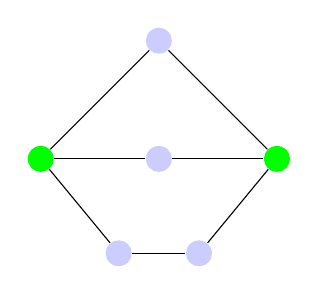
\begin{tikzpicture}
[scale=0.3,auto=center,every node/.style={circle,fill=blue!20}]
  
  \node (n1) at (0,5) [fill=green] {};
  \node (n6) at (10,5) [fill=green] {};
  \node (n2) at (5,10)  {};
  \node (n3) at (5,5)  {};
  \node (n4) at (3.3,1)  {};
  \node (n5) at (6.7,1)  {};

  \foreach \from/\to in {n1/n2,n2/n6,n3/n1,n3/n6, n1/n4, n4/n5, n5/n6}
    \draw (\from) -- (\to);

\end{tikzpicture}
    \end{center}

\end{column}
\begin{column}{5cm}
\begin{center}
A $\theta_{2,2,3,3,4,5}$ graph
\\[0.2cm]
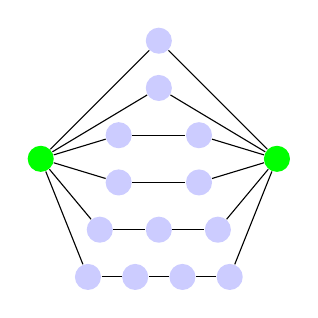
\begin{tikzpicture}
[scale=0.3,auto=center,every node/.style={circle,fill=blue!20}]
  
  \node (n1) at (0,5) [fill=green] {};
  \node (n2) at (10,5) [fill=green] {};
  \node (n3) at (5,10)  {};
  \node (n4) at (5,8)  {};
  \node (n5) at (3.3,6)  {};
  \node (n6) at (6.7,6)  {};
  \node (n7) at (3.3,4)  {};
  \node (n8) at (6.7,4)  {};
  \node (n9) at (2.5,2)  {};
  \node (n10) at (5,2)  {};
  \node (n11) at (7.5,2)  {};

  \node (n12) at (2,0)  {};
  \node (n13) at (4,0)  {};
  \node (n14) at (6,0)  {};
  \node (n15) at (8,0)  {};

  \foreach \from/\to in {n1/n3,n3/n2,n1/n4,n4/n2, n1/n5,n5/n6,n6/n2,n1/n7,n7/n8,n8/n2,n1/n9,n9/n10,n10/n11,n11/n2, n1/n12,n12/n13,n13/n14,n14/n15,n15/n2}
    \draw (\from) -- (\to);
\end{tikzpicture}
\end{center}
\end{column}
\end{columns}

\begin{equation*} 
 \frac{x - 1}{x^{t-1}}\Biggl(\prod_{j=1}^{t} \bigl((x-1)^{a_j}-(-1)^{a_j}\bigl) + (x - 1)^{t-1}\prod_{j=1}^{t} \bigl((x-1)^{a_j - 1}+(-1)^{a_j}\bigl)\Biggl)
\end{equation*}


\end{frame}

\begin{frame}
\frametitle{What has been done one this so far?}
Investigations regarding Galois groups of theta graphs have been done by Kerri Morgan and Daniel Delbourgo in a number of papers, primarily:
\bibitem{morgan} K. Morgan,  Galois groups of chromatic polynomials, {\em LMS J. Comput. Math.} 15, p.281–307 (2012).
\bibitem{delbourgo-morgan} D. Delbourgo and K. Morgan, Algebraic invariants arising from the chromatic polynomials of theta graphs, {\em Australas. J. Combinatorics} 59, p.293–310 (2014)


\end{frame}

\begin{frame}[shrink=20]
\frametitle{Summary of results on Galois groups of theta graphs}
1. K. Morgan (amongst other results) calculated Galois groups for all theta graphs with chromatic polynomials with degree at most 19. The results are presented in a number of tables, split by dimension of number of irreducible factors in chromatic polynomial factorisation, chromatic number of the graphs, 

2. K. Morgan and D. Delbourgo derive and \textbf{formally prove} a general formula for Galois groups of theta graphs of the form $\theta_{a,a,a}$ and $\theta_{a,a,a}$.
\begin{equation*}
Gal(K_{P(\theta_{a,a+1,a+2},\lambda)} / \mathbb{Q}) \cong \begin{cases}
			(\mathbb{Z}/(a^2+a)\mathbb{Z})^{\times} \times S_{a+1}, & \text{if } a \not\equiv 1 \text{ ( mod 3)} \\
            (\mathbb{Z}/(a^2+a)\mathbb{Z})^{\times} \times  C_2 \times S_{a-1}, & \text{if } a \equiv 1 \text{ ( mod 3)}
		 \end{cases} 
\end{equation*}



\begin{equation*}
\tcbhighmath[drop fuzzy shadow]{Gal(K_{P(\theta_{a,a,a},\lambda)} / \mathbb{Q}) \cong S_{3(a-1)}}
\end{equation*}

3. The authors conjecture and perform extensive numerical verification for the closed form formula for a general theta graph with arbitrary path lengths.
\begin{equation}
Gal(K_{P(\theta_{a_1,a_2,a_3},\lambda)}/\mathbb{Q}) \cong 
(\mathbb{Z}/N_{a_1,a_2,a_3}\mathbb{Z})^{\times} \times S_{a_1+a_2+a_3-2 - \sum_{d \in \sum }\phi(d) }
\end{equation}
where  the integer $N_{a_1,a_2,a_3}=lcm_{d \in \sum_{a_1,a_2,a_3}}(d)$.


\end{frame}

\begin{frame}[shrink=20]
\frametitle{Extension to some generalised theta graphs}
\textbf{Step 1}. In the thesis I focused on generalised theta graphs with 4 paths \textbf{theta-4}, and generalised theta graphs with 5 paths \textbf{theta-5}. With the help of magma package I performed calculations of Galois groups for all theta-4 and theta-5 graphs with chromatic polynomials of degree no greater than 19, and presented the results in a similar fashion as in K.Morgan work. \\
(A) The code can be reused for any other family of graphs with chromatic polynomials available in closed form with minimal enhancements required.\\
(B) Not surprisingly the results quickly become quite complex for deriving a general pattern.

\textbf{Step 2}. I further restricted my attention to generalised theta graphs with same path lengths. \textbf{$\Theta^{(s,p)}$} is a generalised theta graphs with p paths of length s. I refer to them as \textbf{Sokal graphs}. 



\begin{columns}
\begin{column}{5cm}
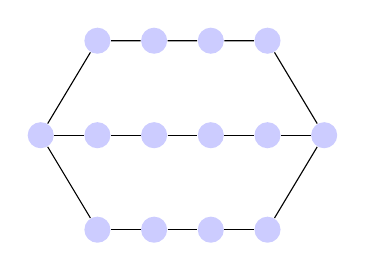
\begin{tikzpicture}
[scale=0.3,auto=center,every node/.style={circle,fill=blue!20}]

  \node (n1) at (0,5) {};
  \node (n6) at (12,5) {};
  \node (n2) at (2.4,9)  {};
  \node (n7) at (4.8,9)  {};
  \node (n8) at (7.2,9) {};
  \node (n9) at (9.6,9) {};
  \node (n3) at (2.4,5)  {};
  \node (n10) at (4.8,5) {};
  \node (n11) at (7.2,5){};
  \node (n12) at (9.6,5){};
  \node (n4) at (2.4,1)  {};
  \node (n13) at (4.8,1) {};
  \node (n14) at (7.2,1){};
  \node (n5) at (9.6,1) {};
  \foreach \from/\to in {n1/n2, n2/n7, n7/n8, n8/n9, n9/n6}
    \draw (\from) -- (\to);
  \foreach \from/\to in {n1/n3, n3/n10, n10/n11, n11/n12, n12/n6}
    \draw (\from) -- (\to);
  \foreach \from/\to in {n1/n4, n4/n13, n13/n14, n14/n5, n5/n6}
    \draw (\from) -- (\to);

\end{tikzpicture}
\begin{center}
$\Theta^{(5,3)}$
\end{center}
\end{column}
\begin{column}{5cm}
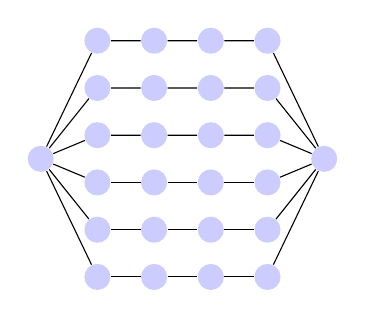
\begin{tikzpicture}
[scale=0.3,auto=center,every node/.style={circle,fill=blue!20}]
  \node (n1) at (0,5) {};
  \node (n6) at (12,5) {};
  \node (n2) at (2.4,10)  {};
  \node (n7) at (4.8,10)  {};
  \node (n8) at (7.2,10)  {};
  \node (n9) at (9.6,10)  {};
  \node (n3) at (2.4,8)   {};
  \node (n10) at (4.8,8)  {};
  \node (n11) at (7.2,8)  {};
  \node (n12) at (9.6,8)  {};
  \node (n4) at (2.4,6)   {};
  \node (n13) at (4.8,6)  {};
  \node (n14) at (7.2,6)  {};
  \node (n5) at (9.6,6)   {};
  \node (n15) at (2.4,4)  {};
  \node (n16) at (4.8,4)  {};
  \node (n17) at (7.2,4)  {};
  \node (n18) at (9.6,4)  {};
  \node (n19) at (2.4,2)  {};
  \node (n20) at (4.8,2)  {};
  \node (n21) at (7.2,2)  {};
  \node (n22) at (9.6,2)  {};
  \node (n23) at (2.4,0)  {};
  \node (n24) at (4.8,0)  {};
  \node (n25) at (7.2,0)  {};
  \node (n26) at (9.6,0)  {};
  \foreach \from/\to in {n1/n2, n2/n7, n7/n8, n8/n9, n9/n6}
    \draw (\from) -- (\to);
  \foreach \from/\to in {n1/n3, n3/n10, n10/n11, n11/n12, n12/n6}
    \draw (\from) -- (\to);
  \foreach \from/\to in {n1/n4, n4/n13, n13/n14, n14/n5, n5/n6}
    \draw (\from) -- (\to);
  \foreach \from/\to in {n1/n15, n15/n16, n16/n17, n17/n18, n18/n6}
    \draw (\from) -- (\to);
  \foreach \from/\to in {n1/n19, n19/n20, n20/n21, n21/n22, n22/n6}
    \draw (\from) -- (\to);
  \foreach \from/\to in {n1/n23, n23/n24, n24/n25, n25/n26, n26/n6}
    \draw (\from) -- (\to);

\end{tikzpicture}
\end{column}
\end{columns}
\end{frame}








\begin{frame}
    \frametitle{Galois Groups of Sokal Graphs $\Theta^{(s,p)}$}
    \footnotesize
    \begin{tabular}{|c|c|c|c|c|c|c|c|}
    \hline
    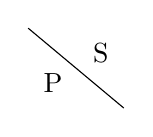
\begin{tikzpicture}[baseline=(current bounding box.center)]
        \node[anchor=south west,inner sep=0,minimum width=1.2cm,minimum height=1cm] (box) at (0,0) {};
        \draw[black] (box.north west) -- (box.south east);
        \node[anchor=south west,xshift=2pt,yshift=2pt] at (box.south west) {P};  % P is now in the bottom-left
        \node[anchor=north east,xshift=-2pt,yshift=-2pt] at (box.north east) {S}; % S is now in the top-right
    \end{tikzpicture} & 2 & 3 & 4 & 5 & 6 & 7 & 8 \\
    \hline
    3  & $S_{3}$ & $S_{6}$  & $S_{9}$  & $S_{12}$ & $S_{15}$ & $S_{18}$ & $S_{21}$ \\ 
    4  & $S_{4}$ & $S_{8}$  & $S_{12}$ & $S_{16}$ & $S_{20}$ & $S_{24}$ & $S_{28}$ \\ 
    5  & $S_{5}$ & $S_{10}$ & $S_{15}$ & $S_{20}$ & $S_{25}$ & $S_{30}$ & $S_{35}$ \\ 
    6  & $S_{6}$ & $S_{12}$ & $S_{18}$ & $S_{24}$ & $S_{30}$ & $S_{36}$ & $S_{42}$ \\ 
    7  & $S_{7}$ & $S_{14}$ & $S_{21}$ & $S_{28}$ & $S_{35}$ & $S_{42}$ & $S_{49}$ \\ 
    8  & $S_{2}$, $S_{6}$  & $S_{16}$ & $S_{24}$ & $S_{2}$, $S_{30}$ & $S_{40}$ & $S_{48}$ & $S_{2}$, $S_{54}$ \\ 
    9  & $S_{9}$  & $S_{18}$ & $S_{27}$ & $S_{36}$ & $S_{45}$ & $S_{54}$ & $S_{63}$ \\ 
    10 & $S_{10}$ & $S_{20}$ & $S_{30}$ & $S_{40}$ & $S_{50}$ & $S_{60}$ & $S_{70}$ \\ 
    11 & $S_{11}$ & $S_{22}$ & $S_{33}$ & $S_{44}$ & $S_{55}$ & $S_{66}$ & $S_{77}$ \\ 
    12 & $S_{12}$ & $C(4), S_{20}$ & $S_{36}$ & $S_{48}$ & $S_{60}$ & $S_{72}$ & $C(4), S_{80}$ \\ 
    13 & $S_{13}$ & $S_{26}$ & $S_{39}$ & $S_{52}$ & $S_{65}$ & $S_{78}$ & $S_{91}$ \\ 
    14 & $S_{2}$, $S_{12}$ & $S_{28}$ & $S_{42}$ & $S_{2}$, $S_{54}$ & $S_{70}$ & $S_{84}$ & $S_{2}$, $S_{96}$ \\ 
    15 & $S_{15}$ & $S_{30}$ & $S_{45}$ & $S_{60}$ & $S_{75}$ & $S_{90}$ & $S_{105}$ \\ 
    16 & $S_{16}$ & $S_{32}$ & $C(6), S_{42}$ & $S_{64}$ & $S_{80}$ & $S_{96}$ & $S_{112}$ \\ 
    \hline
    \end{tabular}
\end{frame}




\begin{frame}[shrink=10]
\frametitle{Galois groups of Sokal graphs $\Theta^{(s,p)}$}

\scriptsize % Reduce the font size
\begin{tabular}{| p{0.03\textwidth} | p{0.05\textwidth} | p{0.08\textwidth} | p{0.1\textwidth} | p{0.1\textwidth} | p{0.04\textwidth} | p{0.04\textwidth} | p{0.1\textwidth} | p{0.06\textwidth} | p{0.1\textwidth} | } % Slightly increased width of last column
    \hline
      & 2 & 3 & 4 & 5 & 6 & 7 & 8 & ... & $s$ \\
    \hline
    3 & $S_{3}$ & $S_{6}$ & $S_{9}$ & $S_{12}$ & $S_{15}$ & $S_{18}$ & $S_{21}$ & ... & $\color{LimeGreen} S_{3(s-1)}$ \\ 
    \hline
    4 & $S_{4}$ & $S_{8}$ & $S_{12}$ & $S_{16}$ & $S_{20}$ & $S_{24}$ & $S_{28}$ & ... & $\color{Magenta} S_{4(s-1)}$  \\ 
    \hline
    5 & $S_{5}$ & $S_{10}$ & $S_{15}$ & $S_{20}$ & $S_{25}$ & $S_{30}$ & $S_{35}$ & ... & $\color{Magenta} S_{5(s-1)}$ \\ 
    \hline
    6 & $S_{6}$ & $S_{12}$ & $S_{18}$ & $S_{24}$ & $S_{30}$ & $S_{36}$ & $S_{42}$ & ... & $\color{Magenta} S_{6(s-1)}$ \\ 
    \hline
    7 & $S_{7}$ & $S_{14}$ & $S_{21}$ & $S_{28}$ & $S_{35}$ & $S_{42}$ & $S_{49}$ & ... & $\color{Magenta} S_{7(s-1)}$ \\ 
    \hline
    8 & $S_{2}, S_{6}$ & $S_{16}$ & $S_{24}$ & $S_{2}, S_{30}$ & $S_{40}$ & $S_{48}$ & $S_{2}, S_{54}$ & ... & ??? \\ 
    \hline
    9 & $S_{9}$ & $S_{18}$ & $S_{27}$ & $S_{36}$ & $S_{45}$ & $S_{54}$ & $S_{63}$ & ... & $\color{BurntOrange} S_{9(s-1)}?$ \\ 
    \hline
    10 & $S_{10}$ & $S_{20}$ & $S_{30}$ & $S_{40}$ & $S_{50}$ & $S_{60}$ & $S_{70}$ & ... & $\color{BurntOrange} S_{10(s-1)}?$ \\ 
    \hline
    11 & $S_{11}$ & $S_{22}$ & $S_{33}$ & $S_{44}$ & $S_{55}$ & $S_{66}$ & $S_{77}$ & ... & $\color{BurntOrange} S_{11(s-1)}?$ \\ 
    \hline
    12 & $S_{12}$ & $C(4), S_{20}$ & $S_{36}$ & $S_{48}$ & $S_{60}$ & $S_{72}$ & $C(4), S_{80}$ & ... & ??? \\ 
    \hline
    13 & $S_{13}$ & $S_{26}$ & $S_{39}$ & $S_{52}$ & $S_{65}$ & $S_{78}$ & $S_{91}$ & ... & $\color{BurntOrange} S_{13(s-1)}?$ \\ 
    \hline
    14 & $S_{2}, S_{12}$ & $S_{28}$ & $S_{42}$ & $S_{2}, S_{54}$ & $S_{70}$ & $S_{84}$ & $S_{2}, S_{96}$ & ... & ??? \\ 
    \hline
    15 & $S_{15}$ & $S_{30}$ & $S_{45}$ & $S_{60}$ & $S_{75}$ & $S_{90}$ & $S_{105}$ & ... & $\color{BurntOrange} S_{15(s-1)}?$ \\ 
    \hline
    16 & $S_{16}$ & $S_{32}$ & $C(6), S_{42}$ & $S_{64}$ & $S_{80}$ & $S_{96}$ & $S_{112}$ & ... & ??? \\ 
    \hline
    \vdots & \vdots & \vdots & \vdots & \vdots & \vdots & \vdots & \vdots & ... & \vdots \\ 
    \hline
    p & ??? & ??? & ??? & ??? & ??? & ??? & ??? & ... & not $\color{red} \cancel{S_{p(s-1)}}$ \\ 
    \hline
\end{tabular}

\end{frame}


\begin{frame}{Summary of what has been done and potential steps for future research}
1. A General magma code has been produced allowing for calculation of Galois groups of some family of graphs for which chromatic polynomial is available in closed form. Results are nice to view tables allowing to see for any patterns in respective Galois groups.
\\
2. These steps have been applied to theta-4 and theta-5 graphs, and respective tables have been produced.
\\
3. Further calculation have been extended to Sokal graphs, or generalised theta graphs with equidistant paths. A sample table has been produced, which facilitates rejection of conjecture that the general formula for a Galois group of Sokal graph is $S_{p(s-1)}$, but support that it is $S_{p(s-1)}$ for some values of p. numerical confirmation performed for p equal to 4, 5, 6, 7. 
    
\end{frame}


\begin{frame}{Potential directions of future research in this area}
1. Completion of formal proof of the Galois group for theta graphs conjectured by Morgan and Delbourgo.
\\
2. Producing a conjecture for general formula of generalised theta graph with equidistant paths, and formal proof for general case or for some specific numbers of paths. 
\\
3. All considerations have been done over the field of rational numbers. As chromatic polynomials are monic polynomials with integer coefficients, it would be possible to perform same analysis over e.g. Finite fields.
\\
4. Extending the analysis to another family of finite graphs for which chromatic polynomial is available in closed form.
\\
5. Extending analysis to other graph polynomials
    
\end{frame}


\end{document}